\section{Candidate code list exploration} 
\label{s:codelistanalyzer}

We describe here a proof-of-concept experiment, which involves query-based exploration of candidate code lists in the LOV knowledge base, in which we can find the description of RDF/S vocabularies and OWL ontologies defined for and used by datasets on the Linked Data Cloud.

The goal of this part of our research has been to create and apply a collection of SPARQL queries that can be used in the process of exploring code lists in LOV. % and other knowledge bases as well. %Another specific goal was to identify the coverage of knowledge instances with respect to their abstract concepts. 

\subsection{Query sequence for candidate code list exploration}
The exploration of candidate code lists in a vocabulary consists of several steps and five main SPARQL queries. The exact parameterized SPARQL queries labeled Q1 through Q5 including the necessary prefixes can also be found on our GitHub repository\footnote{\url{https://github.com/nvbach91/iga-hybrid}}.

The general steps of this experiment are summarized as follows:

\begin{enumerate}
    \item Make a list of vocabularies that might contain code lists, sorted by the number of included individuals and classes.

    \item In each vocabulary, find all classes and count the number of their instances.% and subclasses.

    \item For each class with at least one instance, find all its instances (individuals) and check if these instances are connected to \emph{skos:Concept} (which is known to be used for codes in code lists).

    \item Query for direct relationships between these instances and use this information to visualize the candidate code list (see e.g. Figure \ref{fig:code-list-visualized})

    \item Query for the instance-instance relationships (assignment properties) that exist in each vocabulary, including the total number of instances on both sides of the relationships (this helps to check if we missed any codes).

\end{enumerate}

Using this procedure, we collect all candidate code lists for further review. If a result proves to be a candidate code list but does not use \emph{skos:Concept}, we enhance it by connecting the collected instances with their classes via the \emph{skos:inScheme} property, and annotating them with \emph{skos:Concept} and \emph{skos:ConceptScheme} classes (using SPARQL UPDATE, see Code listing \ref{lst:sparql6}). The enhanced data are then compiled into one knowledge base, which provides simpler and more straightforward access to the candidate code lists thanks to SKOS.



Note that none of the queries is to be understood as a strict definition of what should be a code list.
Instead, the queries assemble collections of results that can be independently inspected and gradually produce a code list knowledge base potentially useful for the community (without guaranteeing that every single element would fully satisfy a rigorous or common-sense concept of what should a code list be).
The queries, especially, Q3 and Q4, are derived from the analysis presented in the previous section. 

\medskip
\medskip
\noindent\textbf{Q1: Identify the named graph IRIs of the target vocabularies}. This step retrieves a list of vocabulary IRIs and their names. In addition, we also query for the number of classes and class instances in each vocabulary.\footnote{Note that here we are using the \textit{GRAPH} keyword to determine the boundaries in which we count the classes and class instances for each vocabulary. This is thanks to the fact that LOV maintains each vocabulary in a separate graph. Another intuitive approach to get the same results is to use the \textit{rdfs:isDefinedBy} property. However, this approach is unreliable because not all vocabularies use this property to define their terms. To make it reliable, we would have to enhance the data by adding it to all the terms in each vocabulary. This can be done using
%keyword some vocabularies are not listed here even though they include class instances. This is because this query assumes the classes have the property \textit{rdfs:isDefinedBy} so that their number can be counted for each vocabulary. This can be fixed by 
query Q0 (available in our GitHub repository) before running query Q1. However, this would require setting up a custom endpoint with SPARQL UPDATE feature enabled. Also, here we only retrieve English labels to not distract the users when browsing the code lists.} In LOV, the total number of vocabularies having at least one class instance is 271 (out of all 818 vocabularies). A part of the results for this query is displayed in Table \ref{tab:q1-results}, which lists the top vocabularies with the highest number of class instances. The number of classes and instances indicates the probability of code lists existing in each vocabulary and helps to set the priority for analyzing each vocabulary. Vocabularies that have a low number of classes and instances will probably be less likely to include code lists. %This way, the analysis procedure would find the majority of code lists in the targeted knowledge base sooner.

\begin{lstlisting}[captionpos=b, caption=Q1 -- Query to get a list of vocabularies with class count and class instance count,label=lst:sparql1,basicstyle=\small\ttfamily,frame=single]
SELECT DISTINCT ?v
 (GROUP_CONCAT(DISTINCT ?vp;separator="|") AS ?vps)
 (GROUP_CONCAT(DISTINCT ?vl;separator="|") AS ?vls)     
 (COUNT (DISTINCT ?c) AS ?nc)
 (COUNT (DISTINCT ?i) AS ?ni)
WHERE {
  ?v a voaf:Vocabulary .
  OPTIONAL { ?v vann:preferredNamespacePrefix ?vp }
  OPTIONAL {
    VALUES ?vlp { rdfs:label skos:prefLabel
                  dc:title dcterms:title }
    ?v ?vlp ?vl .
    FILTER(LANGMATCHES(LANG(?vl), 'en') ||
           LANGMATCHES(LANG(?vl), '')) }
  OPTIONAL {
    GRAPH ?v {
      VALUES ?class { owl:Class rdfs:Class } .
      ?c a ?class . OPTIONAL { ?i a ?c } } }
} GROUP BY ?v ORDER BY DESC(?ni)
\end{lstlisting}

\begin{table}[h]
\footnotesize
\centering
\begin{tabular}{|l|l|r|r|}
\hline
\textbf{\texttt{?vps}} & \textbf{\texttt{?vls}}                  & \textbf{\texttt{?nc}} & \textbf{\texttt{?ni}} \\ \hline
\hline
\textbf{Prefix} & \textbf{Label}                                 & \textbf{Class} & \textbf{Inst.} \\ \hline
losp       & Linked open specialities RF                         & 6              & 2\,009 \\ \hline
cfp        & Climate and Forecast standard                       & 48             & 1\,972 \\ \hline
cff        & Climate and Forecast features                       & 48             & 1\,666 \\ \hline
oum        & Ontology of units of Measure                        & 1\,078         & 1\,601 \\ \hline
ifc        & IFC4\_ADD1                                          & 1\,395         & 1\,155 \\ \hline
cwrc       & The CWRC Ontology                                   & 124            & 823  \\ \hline
gn         & The Geonames ontology                               & 7              & 699  \\ \hline
ids        & IDS Information Model                               & 290            & 675  \\ \hline
mil        & The Muninn Military Ontology                        & 142            & 667  \\ \hline
semsur     & SemSur, Version 2.0                                 & 3\,890         & 329  \\ \hline
common     & The Delivery Context Ontology                       & 150            & 314  \\ \hline
geop       & Geopolitical Ontology                               & 11             & 312  \\ \hline
uniprot    & Uniprot Core Ontology                               & 252            & 312  \\ \hline
obo        & Ontology for Biomedical Investi.                    & 5\,374         & 296  \\ \hline
%ceo        & CEO: Consumer Electronics Ont.                      & 49             & 285  \\ \hline
%lexinfo    & LexInfo                                             & 279            & 275  \\ \hline
%odrl       & ODRL Version 2.2                                    & 45             & 239  \\ \hline
%aos        & Sex, Genders, Preferences and                       & 39             & 237  \\ \hline
%topo       & An ontology for describing terri.                   & 52             & 226  \\ \hline
%jup        & Ontology of Building Accessib.                     & 48             & 206  \\ \hline
%geosp      & GeoSpecies Ontology                                & 86             & 204  \\ \hline
%vin        & Wine Ontology                                      & 101            & 161  \\ \hline
%cbo        & Comic Book Ontology                                & 68             & 138  \\ \hline
%sw-quality & SQuAP Ontology                                     & 153            & 135  \\ \hline
%uby        & ubyCat.owl                                         & 53             & 134  \\ \hline
%pmovn      & Predicate Model for Ontologies                     & 53             & 133  \\ \hline
%modsci     & ModSci, Modern Science Ontology                    & 244            & 130  \\ \hline
%scoro      & Scholarly Contributions and Roles                  & 20             & 125  \\ \hline
%schema     & Schema.org vocabulary                              & 625            & 124  \\ \hline
%chord      & The Chord Ontology                                 & 9              & 108  \\ \hline
%turismo    & Ontology of Tourist for Saragossa town hall.       & 51             & 102  \\ \hline
%rsctx      & Recommender System Context                         & 52             & 91   \\ \hline
%ddesc      & Denotative Description Ontology (ArCo network)     & 66             & 91   \\ \hline
%citof      & CiTOFunction                                       & 6              & 84   \\ \hline
%sh         & W3C Shapes Constraint Language (SHACL) Vocabulary  & 40             & 79   \\ \hline
%s4watr     & SAREF extension for water                          & 72             & 78   \\ \hline
%gold       & General Ontology for Linguistic Description        & 502            & 76   \\ \hline
%voag       & Vocabulary Of Attribution and Governance           & 65             & 76   \\ \hline
%iot-tta    & Ontology for Internet of Things Technologies, Too  & 152            & 76   \\ \hline
%pext       & Proton Ontology                                    & 488            & 72   \\ \hline
%mv         & MobiVoc: Open Mobility Vocabulary                  & 38             & 68   \\ \hline
%sdmx-code  & SDMX Code                                          & 9              & 66   
\end{tabular}
\caption{Q1 sample result (formatted)} \label{tab:q1-results}.
%\vspace{-6mm}
\end{table}

\medskip
\noindent\textbf{Q2: Get a list of instantiated classes with the number of their instances}. From a vocabulary (whose IRI is the parameter of this query), we retrieve classes that have at least one instance. The number of instances indicates the possible size of the candidate code list. We assume that the code list members could be referenced by other entities; we thus also query for the incoming property edge (assignment property) and its domain entity. This means that the class can be the value of \textit{rdfs:range} of the assignment property. We can observe in the query results that not many candidate code lists have an assignment property. % and we presume that these instances are probably not meant to be code lists. They could be just exemplary instances added to the ontology for the illustration of the classes, or because they are considered important in the domain. These cases should be further analyzed based on the meanings of these instances. 
Result examples for query Q2 are displayed in Table \ref{tab:q2-results}.

\begin{lstlisting}[captionpos=b, caption=Q2 -- Query to get the number of instances of each class in an ontology with their range properties and domain classes,label=lst:sparql2,basicstyle=\small\ttfamily,frame=single]
SELECT ?d ?p ?c (COUNT(DISTINCT ?i) AS ?ni)
FROM <${vocab}>
WHERE {
  VALUES ?class { rdfs:Class owl:Class }
  ?c a ?class .
  ?i a ?c .
  OPTIONAL { 
    ?p rdfs:range ?c . 
    OPTIONAL { ?p rdfs:domain ?d }
  }
} GROUP BY ?d ?p ?c ORDER BY DESC(?ni)
\end{lstlisting}

\begin{table}[ht]
\footnotesize
\centering
\begin{tabular}{|l|l|l|r|}
\hline
\textbf{\texttt{?d}}      & \textbf{\texttt{?p}} & \textbf{\texttt{?c}} & \textbf{\texttt{?ni}} \\ \hline
\hline
\textbf{Domain}  & \textbf{Property} & \textbf{Code list} & \textbf{Codes} \\ \hline
mil:PostToUnit   & mil:toUnit        & mil:MilitaryRank           & 605              \\ \hline
foaf:Person      & mil:heldRank      & mil:MilitaryRank           & 605              \\ \hline
org:Organizat.   & mil:rankOf        & mil:MilitaryRank           & 605              \\ \hline
                 &                   & mil:Rank                   & 45               \\ \hline
                 &                   & mil:Soldier                & 34               \\ \hline
                 &                   & mil:MilitaryTrade          & 18               \\ \hline
                 &                   & mil:MilitaryAppo.          & 14               \\ \hline
                 &                   & mil:ArmsType               & 8                \\ \hline
                 &                   & mil:BattleSpace            & 5                \\ \hline
                 &                   & mil:Non-Combat.            & 2                \\ \hline
                 &                   & mil:Role                   & 1                \\ \hline
\end{tabular}
\caption{Q2 sample result for the Military ontology (formatted)} \label{tab:q2-results}
%\vspace{-6mm}
\end{table}

\medskip
\medskip
\medskip
\noindent\textbf{Q3: Get a list of candidate code list members}. This query gives us an overview of all members of the candidate code lists. Here, we retrieve the instances %and subclasses 
of each class in each vocabulary. The vocabulary and the class are the two parameters of this query. The query results are not yet considered code lists but are understood as a mixture of class instances found inside each ontology. In this query, we also look for whether a code list member is tagged with \emph{skos:Concept}. The fact that the class instances are annotated with \emph{skos:Concept} makes it easier to reference them from other knowledge graphs; thanks to \emph{skos:Concept}, the code list can be effectively extracted as a standalone resource (described in Section \ref{s:skos_codelist_collecting}). Examples of results for this query are displayed in Table \ref{tab:q3-results}.

\begin{lstlisting}[captionpos=b, caption=Q3 -- Query to get a list of candidate code list members and whether they are tagged with \textit{skos:Concept} and \textit{skos:inScheme},label=lst:sparql3,basicstyle=\small\ttfamily,frame=single]
SELECT DISTINCT ?i (BOUND(?sc) AS ?bsc)
                   (BOUND(?scs) AS ?bscs)
FROM <${vocab}>
WHERE {
  ?i a <${class}> .
  OPTIONAL { BIND(skos:Concept AS ?sc) .
             ?i a ?sc . }
  OPTIONAL { ?i skos:inScheme ?scs .
             ?scs a skos:ConceptScheme . }
}
\end{lstlisting}

\begin{table}[h]
\footnotesize
\centering
\begin{tabular}{|l|c|c|}
\hline
\textbf{\texttt{?i}}      & \textbf{\texttt{?bsc}} & \textbf{\texttt{?bscs}}      \\ \hline \hline
\textbf{Instance}         & \textbf{skos:Concept}  & \textbf{skos:inScheme}       \\ \hline
mil:1AIFRankCaptain       & Yes                    & No                           \\ \hline
mil:1AIFRankGunner        & Yes                    & No                           \\ \hline
mil:1AIFRankPrivate       & Yes                    & No                           \\ \hline
mil:1AIFRankEngineer      & Yes                    & No                           \\ \hline
mil:1AIFRankNurse         & Yes                    & No                           \\ \hline
mil:1AIFRankCorporal      & Yes                    & No                           \\ \hline
mil:1AIFRankTrooper       & Yes                    & No                           \\ \hline
mil:1AIFRankChaplain      & Yes                    & No                           \\ \hline
mil:1AIFRankSergeant      & Yes                    & No                           \\ \hline
mil:1AIFRankDriver        & Yes                    & No                           \\ \hline
mil:1AIFRankMajor         & Yes                    & No                           \\ \hline
mil:1AIFRankSapper        & Yes                    & No                           \\ \hline
mil:1AIFRankSignaller     & Yes                    & No                           \\ \hline
mil:1AIFRankLieutenant    & Yes                    & No                           \\ \hline
mil:1AIFRankAirMechanic   & Yes                    & No                           \\ \hline
mil:1AIFRankAbleSeaman    & Yes                    & No                           \\ \hline
mil:1AIFRankBombardier    & Yes                    & No                           \\ \hline
\end{tabular}
\caption{Q3 sample result for class \textit{mil:Soldier} in the Military ontology (formatted)} \label{tab:q3-results}
%\vspace{-6mm}
\end{table}

\medskip
\noindent\textbf{Q4: In each candidate code list, get all code list members' data including the relationships between them}. This step is to construct and visualize the candidate code list. For this, we need to query all information about the code list members. As we have mentioned before, a code list can simply have a flat structure, but it can also form a shallow hierarchy via properties such as \textit{skos:broader} or \textit{rdfs:subClassOf}\footnote{\label{note:owlSubClass}The properties \textit{owl:subClassOf} and \textit{owl:subClass} do not exist in the OWL specification, they are however used in the Military ontology. This is probably a mistake made by the authors. We understand that these properties should be \textit{skos:broader} or \textit{rdfs:subClassOf} according to the meanings of the codes, similarly in the case of \textit{org:rankEquivalentTo}, \textit{org:rankSeniorToTransitive}, \textit{org:rankJuniorToTransitive} in Table \ref{tab:q5-results} and some others}. The query results in Table 4 show an example of this particular finding in the Military ontology. To show that this approach can be applied to any vocabulary, Figure \ref{fig:code-list-with-hierarchy} shows the visualization of a code list structure about weekdays from the GoodRelations ontology.


\begin{lstlisting}[captionpos=b, caption=Q4 -- Query to get candidate code list structure,label=lst:sparql4,basicstyle=\small\ttfamily,frame=single]
SELECT DISTINCT ?cn ?i1 ?i1n ?p ?i2 ?i2n
FROM <${vocab}> WHERE {
  ?i1 a <${class}> .
  VALUES ?lp { rdfs:label skos:prefLabel
               dc:title dcterms:title }
  OPTIONAL {
    <${class}> ?lp ?cn . 
    FILTER(LANGMATCHES(LANG(?cn), 'en'))
  }
  OPTIONAL {
    ?i1 ?lp ?i1n . 
    FILTER(LANGMATCHES(LANG(?i1n), 'en'))
  }
  OPTIONAL {
    ?i2 a <${class}> . ?i1 ?p ?i2 .
    OPTIONAL { 
      ?i2 ?lp ?i2n . 
      FILTER(LANGMATCHES(LANG(?i2n), 'en'))
    }
  }
} ORDER BY ?i1
\end{lstlisting}

\begin{table}[ht]
\footnotesize
\centering
\begin{tabular}{|l|l|l|}
\hline
\textbf{\texttt{?i1}}       & \textbf{\texttt{?p}}                     & \textbf{\texttt{?i2}}       \\ \hline \hline
\textbf{Code 1}             & \textbf{Relationship}                    & \textbf{Code 2}             \\ \hline
2nd Corporal                &                                          &                             \\ \hline
2nd Lieutenant              & owl:subClassOf\cref{note:owlSubClass}    & Lieutenant                  \\ \hline
Able Seaman                 &                                          &                             \\ \hline
Air Mechanic                &                                          &                             \\ \hline
Air Mechanic Class I        & owl:subClassOf\cref{note:owlSubClass}    & Air Mechanic                \\ \hline
Air Mechanic Class II       & owl:subClassOf\cref{note:owlSubClass}    & Air Mechanic                \\ \hline
Lieutenant                  &                                          &                             \\ \hline
Sapper                      &                                          &                             \\ \hline
Sergeant                    &                                          &                             \\ \hline
Sergeant Major              &                                          &                             \\ \hline
Signaler                    &                                          &                             \\ \hline
Staff Sergeant              &                                          &                             \\ \hline
\end{tabular}
\caption{Q4 sample result for class \textit{mil:Soldier} in the Military ontology (formatted)} \label{tab:q4-results}
%\vspace{-6mm}
\end{table}

\medskip
\noindent\textbf{Q5: Get a list of distinct properties that connect two code list members}. Optionally, we can verify our results using an additional query that will retrieve all properties connecting the two code list members. Examples of the results for this query are shown in Table \ref{tab:q5-results} which includes the number of connected subjects and objects via a particular predicate.

\begin{lstlisting}[captionpos=b, caption=Q5 -- Query to get a list of properties that connect class instances (also shows the number of instances on both sides),label=lst:sparql5,basicstyle=\small\ttfamily,frame=single]
SELECT (COUNT(DISTINCT ?i1) AS ?ni1) ?p 
       (COUNT(DISTINCT ?i2) AS ?ni2)
FROM <${vocab}> WHERE {
  VALUES ?class { owl:Class rdfs:Class }
  ?c1 a ?class .
  ?c2 a ?class .
  ?i1 a ?c1 .
  ?i2 a ?c2 .
  ?i1 ?p ?i2 .
} GROUP BY ?p
\end{lstlisting}


\begin{table}[h]
\footnotesize
\centering
\begin{tabular}{|r|l|r|}
\hline
\textbf{\texttt{?ni1}}     & \textbf{\texttt{?p}}                  & \textbf{\texttt{?ni2}} \\ \hline \hline
\textbf{Subj. Codes}       & \textbf{Property}                     & \textbf{Obj. Codes}    \\ \hline
384                        & owl:subClass\cref{note:owlSubClass}   & 130                    \\ \hline
41                         & org:rankEquivalentTo*                 & 41                     \\ \hline
39                         & mil:rankOf                            & 5                      \\ \hline
36                         & org:rankJuniorToTransitive*           & 35                     \\ \hline
35                         & org:rankSeniorToTransitive*           & 36                     \\ \hline
33                         & skos:inScheme                         & 5                      \\ \hline
32                         & owl:subClassOf\cref{note:owlSubClass} & 27                     \\ \hline
1                          & owl:disjointWith                      & 1                      \\ \hline
1                          & skos:broader                          & 1                      \\ \hline
\end{tabular}
\footnotesize
\caption{Q5 results for the Military ontology (formatted)\\ \**\textit{these properties do not exist in the Core Organization ontology}} \label{tab:q5-results}
%\vspace{-6mm}
\end{table}


\begin{figure}[h]
\centering
%\captionsetup{justification=centering}
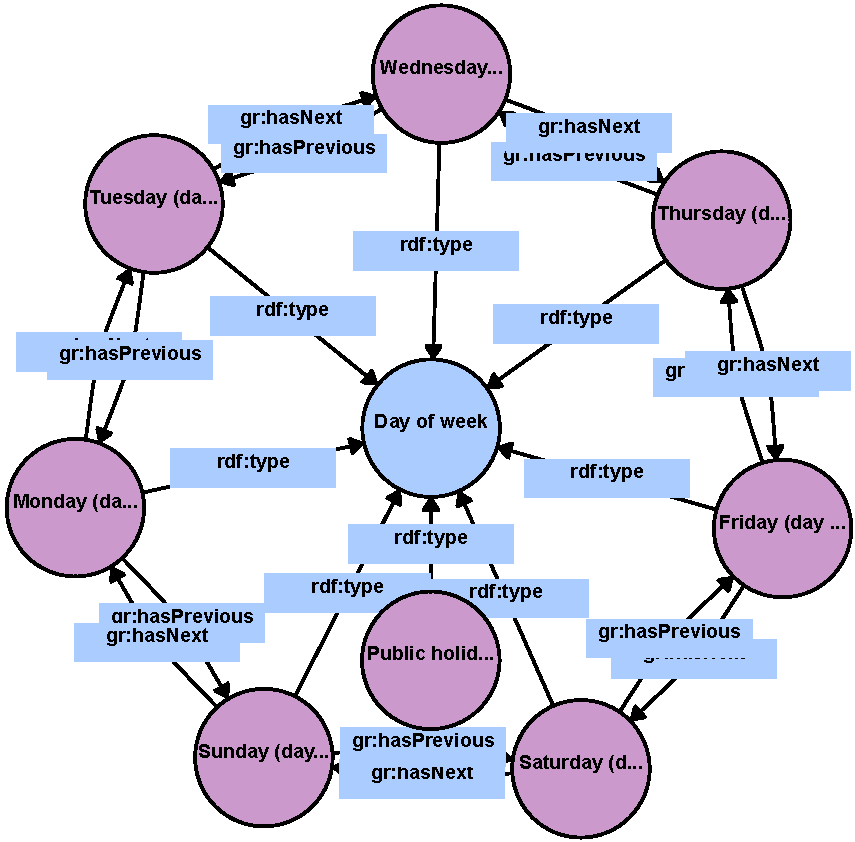
\includegraphics[width=8cm]{figures/code-list-days-of-week}
\caption{Visualization of a simple code list that forms a hierarchy in the GoodRelations vocabulary}
\label{fig:code-list-with-hierarchy}
%\vspace{-4mm}
\end{figure}

\subsection{Implementation: Code List Analyzer}

To make the process of browsing candidate code lists more user-oriented, we have created a web application called Code List Analyzer, which implements the SPARQL queries in our workflow to enable more comprehensive analysis and to provide empirical insight into the queried data. The source code of this application is available on our GitHub\footnote{\label{github-repo}\url{https://github.com/nvbach91/iga-hybrid}} repository under an open-source license. The web client of Code List Analyzer is accessible online via the following link: \url{https://fcp.vse.cz/iga-hybrid}.

\subsection{Exploration results}

The above sequence of SPARQL queries Q1 through Q5 is implemented in our Code List Analyzer tool and has been successfully executed on a total of 818 LOV vocabularies. % (that have at least one class instance). 
We have discovered in aggregation\footnote{\url{https://github.com/nvbach91/iga-hybrid/tree/master/aggregate} (includes scripts to reproduce the results)} that 567 vocabularies do not have any code lists embedded in them. %, probably because these vocabularies are small. 
In 251 of the processed vocabularies, there are structures embedded that resemble code lists. The total number of candidate code lists detected in these vocabularies is 1\,690 and the total number of candidate code list members is 21\,747.

The top vocabularies that have the highest number of candidate code lists and the top vocabularies that have the highest number of code list members along with their SKOS status are listed in Table \ref{tab:top-codes}. There are only 16 vocabularies that use SKOS to model the instances.

\begin{table}[h]
\footnotesize
\begin{tabular}{|l|r|l|}
\hline
\textbf{Vocab} & \textbf{CLists} & \textbf{SKOS} \\ \hline
ifc       & 206         & No   \\ \hline
common    & 79          & No   \\ \hline
obo       & 50          & No   \\ \hline
cfp       & 48          & No   \\ \hline
cff       & 47          & No   \\ \hline
lexinfo   & 41          & No   \\ \hline
vin       & 39          & No   \\ \hline
oum       & 38          & No   \\ \hline
ids       & 37          & Yes  \\ \hline
semsur    & 37          & No   \\ \hline
ceo       & 36          & No   \\ \hline
ontosec   & 31          & No   \\ \hline
modsci    & 31          & No   \\ \hline
iot-tta   & 27          & No   \\ \hline
geosp     & 24          & No   \\ \hline
aos       & 24          & No   \\ \hline
voag      & 22          & No   \\ \hline
gc        & 22          & No   \\ \hline
%...       & ...         & ...   \\ \hline
%uby       & 20          & No   \\ \hline
%cwrc      & 19          & Yes  \\ \hline
%bevon     & 18          & No   \\ \hline
%fowl      & 18          & No   \\ \hline
%turismo   & 15          & No   \\ \hline
%qudt      & 14          & No   \\ \hline
%cbo       & 14          & No   \\ \hline
%topo      & 13          & Yes  \\ \hline
%ldr       & 13          & No   \\ \hline
%scoro     & 12          & No   \\ \hline
%maso      & 12          & No   \\ \hline
%security  & 12          & No   \\ \hline
%cdesc     & 12          & No   \\ \hline
%dk        & 12          & Yes  \\ \hline
%cwmo      & 11          & No   \\ \hline
%ocds      & 11          & No   \\ \hline
%sims      & 10          & No   \\ \hline
%s4watr    & 10          & No   \\ \hline
%bimerr-op & 10          & No   \\ \hline
%rsctx     & 10          & No   \\ \hline
%akt       & 9           & No   \\ \hline
%gr        & 9           & No   \\ \hline
%mil       & 9           & Yes  \\ \hline
%ddesc     & 9           & No   \\ \hline
\end{tabular}
\,
\begin{tabular}{|l|r|l|}
\hline
\textbf{Vocab} & \textbf{Codes} & \textbf{SKOS} \\ \hline
losp           & 2009 & No  \\ \hline
cfp            & 1974 & No  \\ \hline
oum            & 1852 & No  \\ \hline
cff            & 1668 & No  \\ \hline
ifc            & 1627 & No  \\ \hline
semsur         & 1158 & No  \\ \hline
cwrc           & 837  & Yes \\ \hline
mil            & 728  & Yes \\ \hline
ids            & 702  & Yes \\ \hline
gn             & 699  & No  \\ \hline
lexinfo        & 669  & No  \\ \hline
geosp          & 429  & No  \\ \hline
uniprot        & 372  & No  \\ \hline
odrl           & 369  & Yes \\ \hline
common         & 349  & No  \\ \hline
geop           & 312  & No  \\ \hline
obo            & 304  & No  \\ \hline
ceo            & 285  & No  \\ \hline
%...            & ...  & ... \\ \hline
%aos            & 242  & No  \\ \hline
%topo           & 233  & Yes \\ \hline
%vin       & 39  & 161  & No  \\ \hline
%cbo       & 14  & 138  & No  \\ \hline
%uby       & 20  & 136  & No  \\ \hline
%*squap    & 4   & 135  & No  \\ \hline
%pmovn     & 6   & 133  & No  \\ \hline
%*modsci   & 31  & 130  & No  \\ \hline
%scoro     & 12  & 125  & No  \\ \hline
%chord     & 5   & 108  & No  \\ \hline
%turismo   & 15  & 102  & No  \\ \hline
%citof     & 5   & 94   & No  \\ \hline
%rsctx     & 10  & 91   & No  \\ \hline
%ddesc     & 9   & 91   & No  \\ \hline
%s4watr    & 10  & 78   & No  \\ \hline
%voag      & 22  & 77   & No  \\ \hline
%*iot-tta  & 27  & 76   & No  \\ \hline
%gold      & 1   & 76   & No  \\ \hline
%spfood    & 8   & 75   & No  \\ \hline
%pext      & 6   & 72   & No  \\ \hline
%mv        & 8   & 68   & No  \\ \hline
%sdmx-code & 7   & 66   & Yes \\ \hline
%nlon      & 5   & 65   & No  \\ \hline
%ontosec   & 31  & 63   & No  \\ \hline
%akt       & 9   & 62   & No  \\ \hline
\end{tabular}
\centering
%\captionsetup{justification=centering}
\caption{Top vocabularies with the highest number of embedded code lists and code list members} %(*ce: consumerelectronics, mv: mobivoc)}
\label{tab:top-codes} 
%\vspace{-6mm}
\end{table}

The number of vocabularies with at least one assignment property is 156. The remaining 662 vocabularies do not contain any assignment properties. The total number of candidate code lists with at least one assignment property is 782 and the total number of candidate code lists without assignment properties is 908.

\begin{table}[h]
\footnotesize
\centering
\begin{tabular}{|l|r|}
\hline
\textbf{Statistics}                                         & \textbf{Value} \\ \hline
Vocabularies                                                & 818            \\ \hline
Vocabularies using SKOS                                     & 16             \\ \hline
Vocabularies with candidate code lists                      & 251            \\ \hline
Vocabularies without candidate code lists                   & 567            \\ \hline
Vocabularies with assignment properties                     & 156            \\ \hline
Vocabularies without assignment properties                  & 662            \\ \hline
Candidate code lists                                        & 1\,690         \\ \hline
Candidate code list members                                 & 21\,747        \\ \hline
Candidate code lists with assignment properties             & 782            \\ \hline
Candidate code lists without assignment properties          & 908            \\ \hline
\end{tabular}
\caption{Statistics of candidate code lists in LOV vocabularies}
\label{tab:lov-code-list-stats} 
\end{table}

\subsection{Complexity of the process}

The overall query complexity of the above SPARQL query sequence can be calculated by multiplying the number of vocabularies, the number of classes, and the number of instances, since we must repeat the queries that retrieve the instances for each class in each vocabulary. The real-world run-time complexity depends on the database storage implementation. In our case, we directly query against the LOV endpoint, which is powered by the Jena Fuseki triplestore \cite{DBLP:journals/semweb/VandenbusscheAP17}. %, this means that the query speed of Code List Analyzer depends on the query endpoint of LOV. In any case, 
LOV also offers data dump in N-Quads format. This data can be uploaded to a triplestore and its SPARQL endpoint can be run on a local machine or a private server. For our analysis and querying purposes, we have set up a Blazegraph\footnote{\url{https://github.com/blazegraph/database}} SPARQL endpoint\cref{github-repo} with the LOV data dump to avoid query-spamming the official LOV server.

Considering pattern matching in SPARQL has $\mathcal{O}(\log{}n)$ complexity, the query Q1 should have $\mathcal{O}(n\log{}n)$ complexity to create a list of vocabularies, however, we also calculate here the number of classes and class instances, the complexity becomes $\mathcal{O}(n^3)$. Since query Q2 also retrieves classes and instances, but depending on the Q1 results (the vocabulary IRI is a parameter of Q2), it will have $\mathcal{O}(n^2)$ complexity. Because of high complexity, these SPARQL queries cannot be combined and must run separately. Therefore, in order to browse the candidate code lists, the users must first select a vocabulary, while having the option to look at the number of class instances, and then select a candidate code list to view the codes.

\subsection{Exploration result visualization}

In our implementation of Code List Analyzer, which can perform these tasks in a semi-automated manner, we have also included WebVOWL \cite{DBLP:journals/semweb/LohmannNHE15} -- an ontology visualization library. The graph visualization helps in obtaining quick insights while viewing the structures of the extracted candidate code lists, especially the relationships between the codes since they are hard to see in tables. We observed that most of the code lists have a flat structure with one class and many individuals on the same instance level as in Figure~\ref{fig:code-list-visualized}.
